\documentclass[pdftex,12pt]{artikel3}
% Compile with:  pdflatex 

% Settings for source listings.
\usepackage[dvips,letterpaper,margin=1.1in]{geometry}
\usepackage{listings,graphicx}
\usepackage{url}    % usage \href{}{}
\usepackage{xcolor}
%% \usepackage{soul}
%% \usepackage{lipsum}
\usepackage{mathtools}
% \newcommand{\myul}[2][black]{\setulcolor{#1}\ul{#2}\setulcolor{black}}
\usepackage{array}
%% \usepackage{multirow}
\usepackage{alltt}
\usepackage{pifont}
\usepackage{courier}
\usepackage{fancyvrb}
\usepackage{enumitem}
\usepackage[hidelinks]{hyperref}   % hide links in hyperref text
\usepackage{cleveref}     % nice table/figure refs. put after hyperref

% sample stuff for tables and figs
%\usepackage{blindtext}

\usepackage{makeidx}      % for makeindex
\usepackage{tocloft}      % for nicely formatted toc, tof, lof
\usepackage{booktabs,longtable,tabu}

\usepackage[utf8]{inputenc}
\usepackage[T1]{fontenc}
\usepackage{imakeidx}
%% preamble

% the tabfigref command outputs a table or figure reference
% with pattern: "Figure N, The Caption," or "Table N, The Caption,"
% Note: output has a trailing comma(,) for phrasing.
\newcommand{\tabfigref}[1]{\autoref{#1}, \nameref{#1},}

\setcounter{tocdepth}{3}
\makeindex[columns=2, title=Alphabetical Index, intoc]

\lstset{tabsize=4,language=Python,showstringspaces=false}

\title{
\begin{center}
\huge{Jupyter Notebook User Document} \\
\huge{CSCI-471-02}\\
\end{center}
\\
\\
\\
\\
\\
\author{} % \author{Jeffery B. Russell} \\
          % \author{Dan Moore}
\date{}   % \date{Febuary 20, 2020} 
}

%% document starts
\begin{document}
\maketitle


\begin{center}
\author{Jeffery B. Russell},
\author{Daniel Moore},
\author{Louden Yandow}

\date{Febuary 20, 2020}
\end{center}

\newpage

\tableofcontents
\addtocontents{toc}{~\hfill\textbf{Page}\par}
\addcontentsline{toc}{section}{\listfigurename} % include lists of figs
\newpage
\listoffigures
\addtocontents{lof}{~\hfill\textbf{Page}\par}

\newpage

\section{Introduction}

Jupyter \index{jupyter} is an open-source web-based notebook tool that you can use as your development environment.
A coding notebook enables you to intermix markdown and code blocks that you can execute in a single document. This is heavily used in the education and research fields because it makes writing reports easy and reproducible. With Jupyter you can create content that has live code, equations, visualizations and explanatory text.

Jupyter Lab extends the basic notebook functionality and provides you a full web environment to work in. Using this interface you can open terminals, manage files, and even tile multiple editors.

Applications of Jupyter Jab:

\begin{itemize}
  \item Quick experimentation
  \item Telling a story with data
  \item Writing a report
  \item Sharing code snippets for education
\end{itemize}

In this document we are going to go over the basic installation and usage of Jupyter Lab for personal use developing python\index{python}. In the advanced usage section we go over how to use Jupyter on a remote server. This is particularly useful when you want to run algorithms on a remote computer.

\section{Installation}

To install, first go to \href{https://jupyterlab.readthedocs.io/en/stable/getting_started/installation.html}{Jupyter Install}\footnote{\url{ https://jupyterlab.readthedocs.io/en/stable/getting_started/installation.html}} for a detailed guide. This user document assumes that you install Jupyter Lab. \textbf{Do Not Only Install Jupyter Notebook. }

\subsection{Prerequisites}
In order to install Jupyter, you must have Python installed. Your version of Python \textbf{must be 3.3 or greater}. As part of having Python, you will also have pip. Click \href{https://www.python.org/downloads/}{here}\footnote{\url{ https://www.python.org/downloads/}} for the latest version of Python.


However, we highly recommend you take the time now to install \href{https://docs.conda.io/projects/conda/en/latest/user-guide/install/}{Conda}\index{anaconda} now because it'll be helpful later one with some of the more advanced features of Jupyter as well as machine learning focused Python.


You should also have either Firefox, Chrome or Safari as these are the only browsers Jupyter\index{jupyter} is currently known to work with.

\subsection{Installation on Linux}
There a two ways of installing Jupyter on Linux.\\
\\
Using pip\index{pip} the command is \textbf{pip install jupyterlab}.\\
\\
Using conda the command is \textbf{conda install -c conda-forge jupyterlab}

\subsection{Installation on Windows}
Installation on Windows is the same as installation on Linux except that you must also add the user-level bin directory if you installed using \textbf{pip install --user}.

\section{Usage}

To run Jupyter Lab, open your computer's command terminal and enter the following command. This will open Jupyter Lab in your default web browser.

\texttt{jupyter lab}

\tabfigref{fig:jupyterlablauncher} is what you will see upon first running Jupyter Lab. Otherwise, it can open to the most recent notebook you were working on.

\begin{figure}[h!]
    \centering
    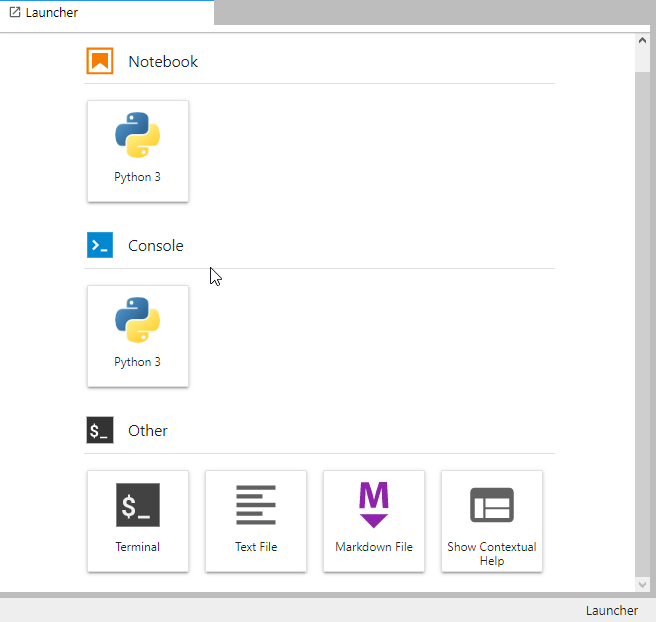
\includegraphics[width=65mm]{launcher.png}
    \caption{Default Jupyter Lab launcher}
    \label{fig:jupyterlablauncher}
\end{figure}

\subsection{Navigation}

Once Jupyter Lab is running, you will see on the left side of the screen a column of icons. Each icon will open a different panel to the right of it when you click it. From top to bottom, these icons have the following functions:
\begin{itemize}
    \item File Browser (folder icon): displays a file browser for the user to open, move, or delete their files.
    \item Running Terminals and Kernels (square stop button inside a circle): shows the user all currently active terminal and kernel sessions.
    \item Commands (palette icon): allows the user to enter various commands into Jupyter Lab.
    \item Notebook Tools (wrench icon): shows various options for the user's current notebook.
    \item Open Tabs (a tabbed window icon): lists all currently open tabs in Jupyter Lab.
\end{itemize}

Additionally, the top toolbar contains the following different drop-down menus: File, Edit, View, Run, Kernel, Tabs, Settings, and Help.

\subsection{Creating a Notebook}

To create a notebook (the working document for both python code and text markdown) from the launcher (\tabfigref{fig:jupyterlablauncher}), click on the Python 3 icon under the orange notebook symbol. Alternatively, if you don't have the launcher open, you can click on File in the toolbar, click New, and finally click Notebook.

This will open an empty, untitled notebook. If you right click on the tab above, or on the name of your notebook in the "Open Tabs" panel on the left, you can rename your notebook.

\subsection{Running a Notebook}

With a notebook open, you can start writing in the editor, the big empty area on the right half of the screen. Just above the editor, you will find the icon to save the open notebook.

There are also a number of icons that directly relate to the "cells" you are writing in. A cell is either python code, markdown, or raw text. You can change what type of text a cell is by clocking on the drop-down menu just above the editor that will say either "Code", "Markdown", or "Raw".

Notebooks work through these cells, in order from top to bottom. The icons above the editor, from left to right, do the following: 

\begin{itemize}
    \item add a cell after the currently selected cell.
    \item cut the currently selected cells.
    \item copy the selected cells.
    \item paste the cells from the clipboard.
    \item run the selected cells and advance to the next cell.
    \item interrupt the kernel.
    \item and restart the kernel.
\end{itemize}

The following example shows how to write code, run code, and insert raw text into the notebook. First, write some python code and click the "Run selected cells and advance" button (circled in red in the figure below). Our output is shown in the next figure (output is given its own unique cell immediately after the cell that produced it).

\begin{figure}[h!]
    \centering
    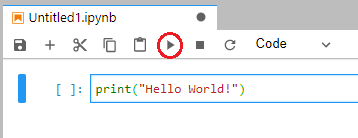
\includegraphics[width=15cm]{code_before_running.png}
    \caption{Code before being run}
    \label{fig:codebeforerunning}
\end{figure}

\begin{figure}[h!]
    \centering
    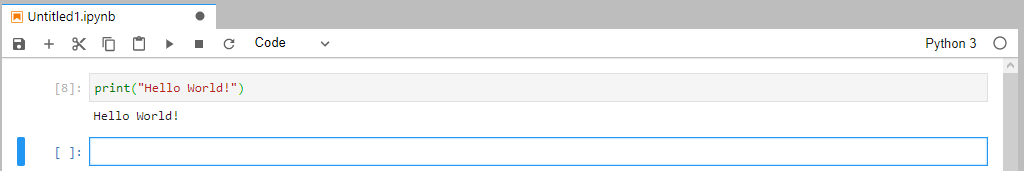
\includegraphics[width=15cm]{code_after_running.png}
    \caption{Code after being run}
    \label{fig:codeafterrunning}
\end{figure}

You can also insert raw text into your document, as shown below. To do this, change the drop-down menu from Code (or Markdown) to Raw, and type what you want in the cell.

\begin{figure}[h!]
    \centering
    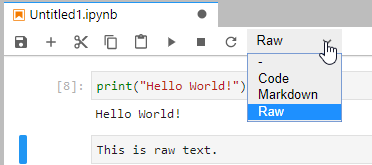
\includegraphics[width=15cm]{raw_text_example.png}
    \caption{Example of raw text}
    \label{fig:rawtextexample}
\end{figure}

\subsection{Exporting Notebooks}
In order to export the document, click the \textbf{File} tab, mouse down to \textbf{Export Notebook As...} and then click any of the myriad of formats to export as that format. The most popular export formats are PDF, Markdown \index{markdown}, and HTML. 

\subsection{Customization}
Customization of Jupyter is in general exceptionally easy.\\
\\
In order to change the theme, one simply needs to go to the \textbf{Settings} tab and drop down to JupyterLab Theme. This will allow you to change from light to dark mode as well as the font sizes for the code, content and UI.\\
\\
Scrolling down the rest of the Settings you see many other things that can be customized.\\
\\
Advanced settings allows you to customize many aspects of Jupyter Lab such as keyboard shortcuts, terminal settings, and a myriad of others. \tabfigref{fig:configuration} shows the configuration menu for Jupyter Lab.

\begin{figure}[h!]
    \centering
    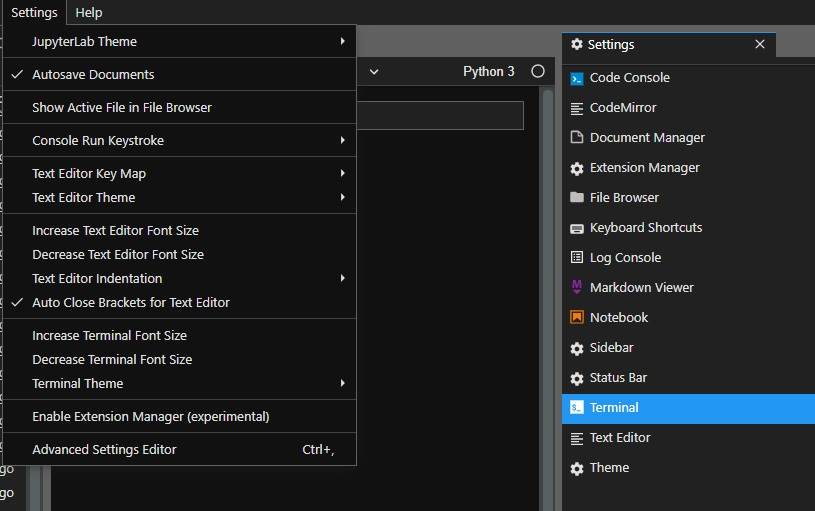
\includegraphics[width=15cm]{settings.jpg}
    \caption{Code after being run}
    \label{fig:configuration}
\end{figure}

\section{Advanced Usage}

In this section we are going to go over how to use multiple programming languages in Jupyter\index{jupyter} and how to connect to your Jupyter Lab instance remotely.

\subsection{Multiple Kernels}

Adding a Kernel in Jupyter enables you to program with another programming language like R\index{r} or Scala\index{scala}.
Up to this point we have been working with the python kernel\index{python} which enables you to make python notebooks. The ability to use multiple kernels is useful for education and having cohesion within one IDE\index{IDE}.

You can view a complete list of kernels here:

\href{https://github.com/jupyter/jupyter/wiki/Jupyter-kernels}{https://github.com/jupyter/jupyter/wiki/Jupyter-kernels}

\begin{figure}[h!]
    \centering
    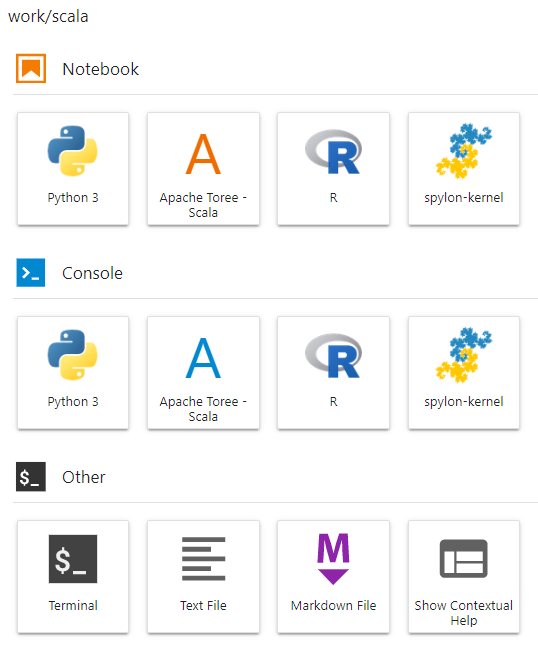
\includegraphics[width=50mm]{exampleKernels.PNG}
    \caption{Example of multiple kernels}
    \label{fig:multKernels}
\end{figure}

\tabfigref{fig:jupyter_server} shows an example of what your launcher would look like with multiple kernels installed.

The most common way to install a kernel is by using the Anaconda\index{anaconda} prompt, pip\index{pip} support is limited here.
Once you start adding multiple kernels, it is best if you start running Jupyter Lab through docker\index{docker} because it would make porting it to another computer easier. A popular docker jupyter lab instance with Scala, Python, and R can be found here:

\href{https://hub.docker.com/u/jupyter/}{https://hub.docker.com/u/jupyter/}

\subsection{Remote Connection}

If you have a firewall Jupyter Lab will only be available on your
local machine at "localhost:8888", however, it is possible to connect to Jupyter Lab from remote computers. 
This is helpful because you can connect to the same Jupyter instance from multiple computers. This would also save you resources on your local computer so you can program on a lightweight chrome-book that would not be able to run a full IDE\index{IDE} like Pycharm\index{pycharm}.

The first step to enable remote host would be to set a password that you can connect to the notebook using. You can set a password that you use to log into the website using the following command:

\texttt{jupyter notebook password}

The Second step would be to launch the Jupyter Lab instance in a headless environment -- it never launches a web browser.

\texttt{jupyter lab --no-browser --port=6000}

The final step is to connect to the Jupyter Lab instance from your
remote computer. The easiest way to do this is via a local port
forward in SSH\index{ssh}. This command essentially forwards all of the traffic on your local machine on a specific port to a remote computer over a ssh connection. The main benefit of doing this is that all the traffic over the connection is encrypted.

\tabfigref{fig:jupyter_server} shows an overview of what the network architecture looks like.


\texttt{ssh -L 6000:localhost:6000 user@remote-host}

\begin{figure}[h!]
    \centering
    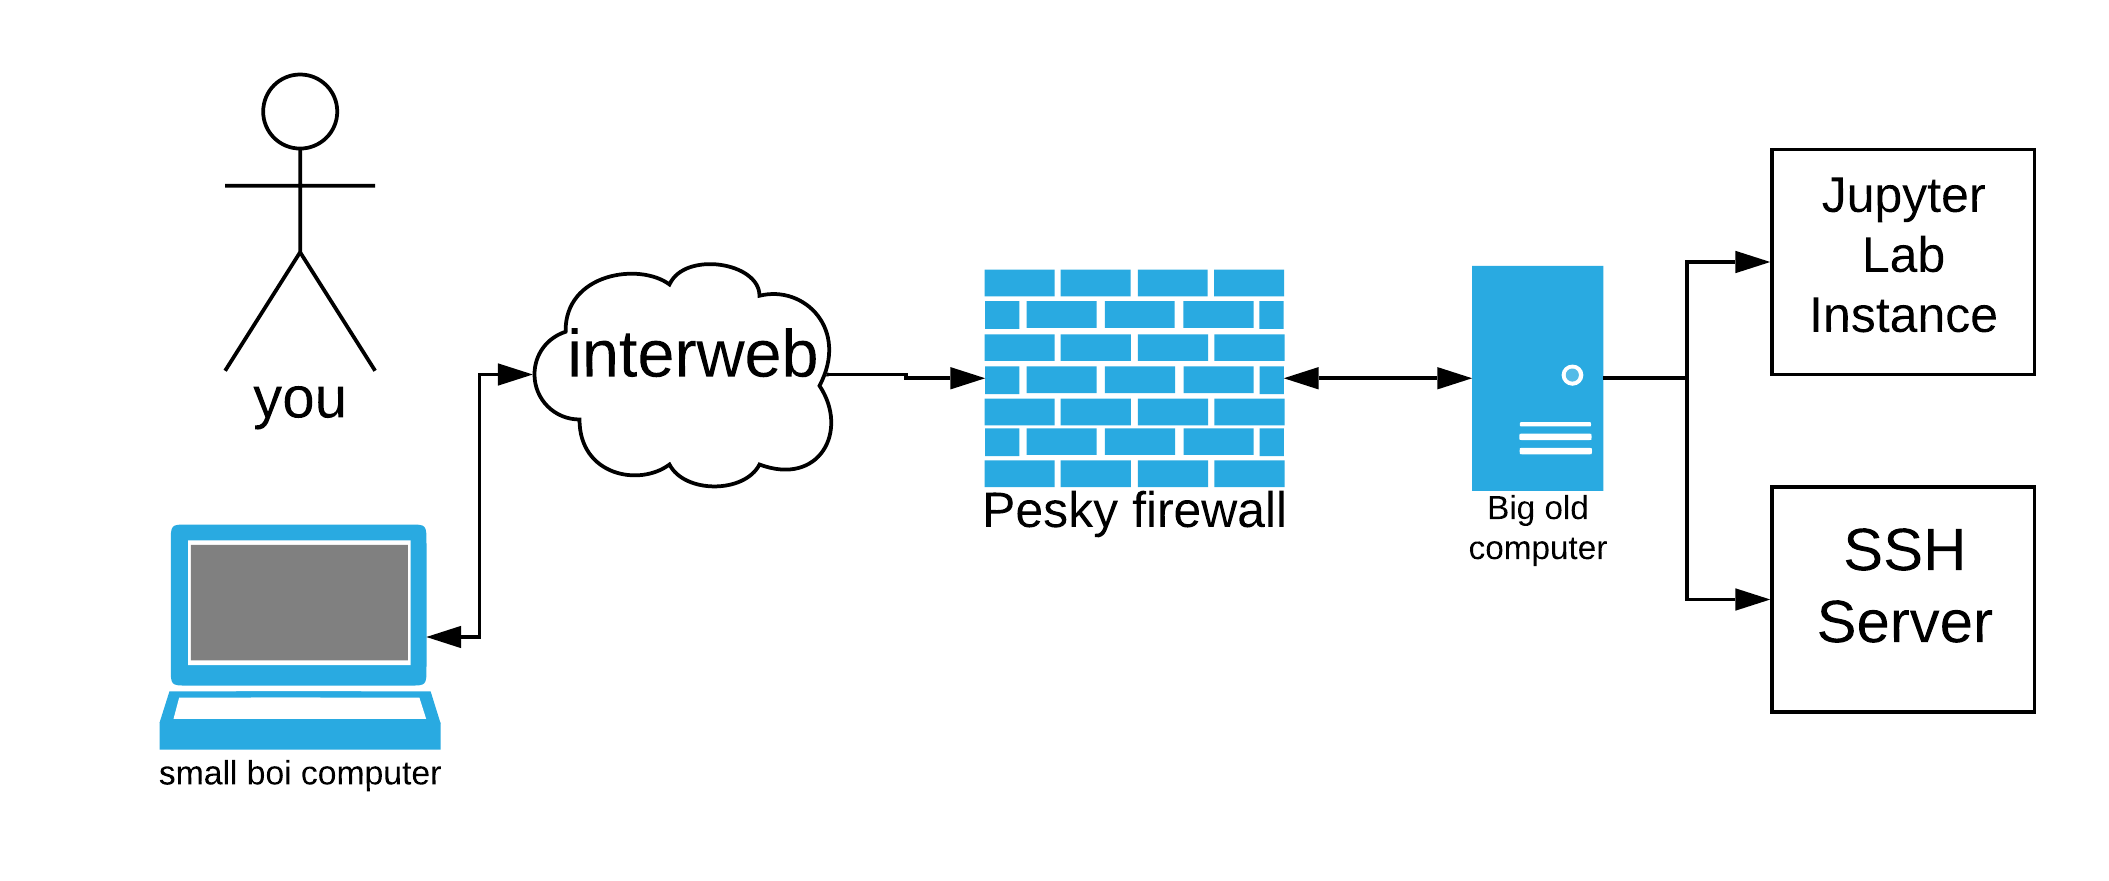
\includegraphics[width=15cm]{remoteJupyter.png}
    \caption{Network Overview}
    \label{fig:jupyter_server}
\end{figure}

After you execute the command above on your remote computer you
would be able to access your Jupyter Lab instance on your computer's "localhost:6000". 

\newpage

\section{Glossary}

\begin{itemize}[label={}]
\item {\bf Anaconda}: Anaconda is a package manager for the R and Python languages aimed towards data science" \footnote{\url{ https://www.anaconda.com}}.\index{anaconda}\\
\item {\bf IDE}: Interactive Development Environment.\index{IDE}\\
\item {\bf Jupyter}: Nonprofit organization created to "develop open-source software, open-standards, and services for interactive computing across dozens of programming languages" \footnote{\url{ https://jupyter.org/}}.\index{jupyter}\\
\item {\bf Markdown(MD)}: Lightweight markup-language \footnote{\url{https://en.wikipedia.org/wiki/Markdown}}.\index{markdown}\\
\item {\bf pip}: Tool for installing and managing python packages \footnote{\url{ https://pypi.org/project/pip/}}.\index{pip}\\
\item {\bf Pycharm}: A popular versitile python IDE developed by \href{https://www.jetbrains.com/}{Jetbrains}.\index{IDE}\\
\item {\bf Python}: High-level interpreted, general purpose programming language \footnote{\url{ https://www.python.org/}}.\index{python}\\
\item {\bf R}: Programming language for statistical computing and graphics \footnote{\url{ https://www.r-project.org/}}.\index{r}\\
\item {\bf Scala}: General purpose functional programming language that runs on the JVM \footnote{\url{ https://scala-lang.org/}}.\index{scala}\\
\item {\bf ssh}: Secure Socket Shell -- used in connecting to a remote computer over a encrypted channel.\index{ssh}\\

\end{itemize}

\newpage

\section{References}

\begin{enumerate}
\item
\url{https://jupyter.org/}
\item
\url{https://www.python.org/}
\item
\url{https://en.wikipedia.org/wiki/Markdown}
\item
\url{https://pypi.org/project/pip/}
\item
\url{https://scala-lang.org/}
\item
\url{https://www.r-project.org/}
\item
\url{https://www.jetbrains.com/}
\end{enumerate}

\newpage

%\section{Index}
\printindex
% outputs its own heading, which does not match the sections

\end{document}